\documentclass
[
	8pt,		% font size
	ngerman,	% hyphenation and more
	a4paper,	% paper size
	landscape,	% orientation
	final		% document status (final/draft)
]{extarticle}

% adjust language %
\usepackage[ngerman]{babel}
% integration of speacial characters %
\usepackage[utf8]{inputenc}
\usepackage[T1]{fontenc}
\usepackage{textcomp}
% adjust page layout %
\usepackage{titlesec}
\usepackage{fancyhdr}
% --------------------------- %
\usepackage{multicol}
\usepackage{multirow}
% --------------------------- %
\usepackage{setspace}
\usepackage{geometry}
\usepackage{adjustbox}
% adjust colors %
\usepackage{color}
% integration of mathematical symbols %
\usepackage{amsmath}
\usepackage{amssymb}
\usepackage{amsthm}
\usepackage{mathtools}
% integration of source code %
\usepackage{listings}
% adjust enumerations %
\usepackage{enumitem}
% adjust tables %
\usepackage{tabularx}
% integration of graphics %
\usepackage{graphicx}
% create graphics %
\usepackage{tikz}
\usetikzlibrary{automata, positioning, arrows}
% integration of seperate files %
\usepackage{standalone}

\usepackage{lmodern}
\DeclareMathOperator{\avg}{avg}

% ========== INFORMATION ========== %
\def\name{Louis Seubert}
\def\prefix{Zusammenfassung}
\def\lecture{Rechnersysteme}
\def\maxpages{6}

% ============== ADJUSTMENTS ============== %
% adjust graphics path %
\graphicspath
{
	{figures/}
}
% adjust page layout %
\geometry
{
	left=0.55cm,
	right=0.55cm,
	top=1.10cm,
	bottom=0.55cm,
	headsep=2mm
}
% adjust source code view %
\lstset
{
	basicstyle=\ttfamily\footnotesize,
	columns=fullflexible,
	numbers=left,						% where to put the line-numbers
	numberstyle=\tiny,  				% the style that is used for the line-numbers
	stepnumber=1,
	numbersep=5pt,						% how far the line-numbers are from the code
	showspaces=false,					% show spaces adding particular underscores
	showstringspaces=false,				% underline spaces within strings
	showtabs=false,						% show tabs within strings adding particular underscores
	frame=none,							% adds a frame around the code
	tabsize=2,							% sets default tabsize to 2 spaces
	captionpos=b,						% sets the caption-position to bottom
	breaklines=true,					% sets automatic line breaking
	breakatwhitespace=false,			% sets if automatic breaks should only happen at whitespace
	xleftmargin=10pt					% left margin to prevent number clipping
}

% make header and footer %
\pagestyle{fancy}
\fancyhead{} % clear header
\fancyhead[L]{\prefix\;\lecture}
\fancyhead[R]{\thepage\;--\;\maxpages}
\fancyhead[C]{\name}
\fancyfoot{} % clear footer

% configure document %
\setitemize{leftmargin=15pt}
\setenumerate{leftmargin=15pt}
\setlist{itemsep=1pt,parsep=1pt,noitemsep}

\setlength{\parindent}{0pt}
\setlength{\parskip}{0pt}
\setlength{\topskip}{10pt}
% set column seperator %
\setlength{\columnseprule}{0.5pt}

% change style %
\titleformat*{\section}{\normalsize\bfseries}
\titlespacing*{\section}{0pt}{4pt}{0pt}

\titleformat*{\subsection}{\small\bfseries}
\titlespacing*{\subsection}{0pt}{4pt}{0pt}

\titleformat*{\subsubsection}{\small\bfseries}
\titlespacing*{\subsubsection}{0pt}{4pt}{0pt}

\titleformat*{\paragraph}{\small\bfseries}
\titlespacing{\paragraph}{0pt}{.5em}{.5em}

\titleformat*{\subparagraph}{\footnotesize\bfseries}
\titlespacing*{\subparagraph}{0pt}{.5em}{.5em}

\newcommand*\important{\par\vspace{\abovedisplayskip}\textbf{Wichtig:}\par}
\newcommand*\example{\par\vspace{\abovedisplayskip}\textbf{Beispiel:}\par}
\newcommand{\includefigure}[1]{\begin{center}\input{#1}\end{center}}

\newenvironment{definitions}{
    \par\vspace{\abovedisplayshortskip}\noindent
    \tabularx{\columnwidth}{>{$}l<{$} @{${}={}$} >{\raggedright\arraybackslash}X}
}{\endtabularx\par\vspace{\belowdisplayshortskip}}

\newcommand{\block}[1]{%
  \raisebox{\dimexpr(\fontcharht\font`X-1em)/2}{\rule{1.4mm}{#1\dimexpr1em/8}}%
}
\DeclareUnicodeCharacter{2581}{\block{1}}
\DeclareUnicodeCharacter{2582}{\block{2}}
\DeclareUnicodeCharacter{2583}{\block{3}}
\DeclareUnicodeCharacter{2584}{\block{4}}
\DeclareUnicodeCharacter{2585}{\block{5}}
\DeclareUnicodeCharacter{2586}{\block{6}}
\DeclareUnicodeCharacter{2587}{\block{7}}
\DeclareUnicodeCharacter{2588}{\block{8}}

\begin{document}
\begin{multicols*}{4}
%\footnotesize
%\fontsize{6}{6}\selectfont
% ======================================================================== %
\section{Protokolle und Stapel}
% ------------------------------------------------------------------------ %
\subsection{OSI-Referenzmodell}
\begin{center}
	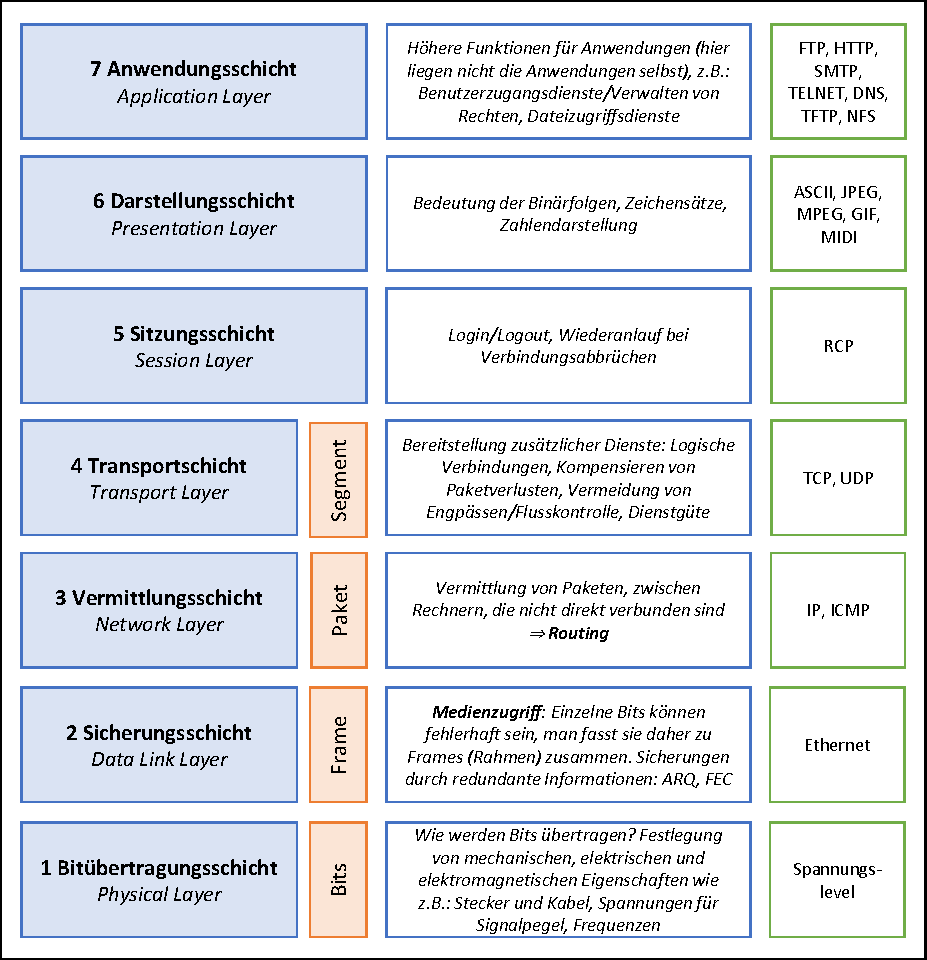
\includegraphics[width=\linewidth]{Documents/OSI.pdf}
\end{center}
% ------------------------------------------------------------------------ %
\subsection{IEEE 802}
\begin{center}
	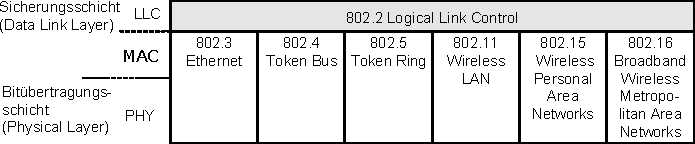
\includegraphics[width=\linewidth]{Documents/IEEE-802.pdf}
\end{center}
\begin{description}
	\item[LLC (Logical Link Control)] 3 Arten von Logical Links:
	      unbestätigt/verbindungslos, bestätigt/verbindungslos,
	      verbindungsorientiert
	\item[MAC (Media Access Control)] Zugriff auf das gemeinsame
	      Medium, z.B.:  CSMA/CD (Ethernet),  CSMA/CA (WLAN)
	\item[PHY] Bitübertragungsschicht
\end{description}
% ------------------------------------------------------------------------ %
\subsection{TCP/IP-Protokollsuite}
\begin{description}
	\item[Anwendungsschicht (Application Layer)]\;\par
	      FTP, HTTP, SMTP, Telnet, DNS, DHCP
	\item[Transportschicht (Transport Layer)]\;\par
	      TCP, UDP
	\item[Internetschicht (Internet Layer)]\;\par
	      IP, ICMP, ARP, Multicast IP, Mobile IP
	\item[Netzwerkschicht (Network Layer)]\;\par
	      SLIP, PPP, Ethernet, Token Ring, WLAN
\end{description}
% ------------------------------------------------------------------------ %
\subsection{Adressierung}
\begin{center}
	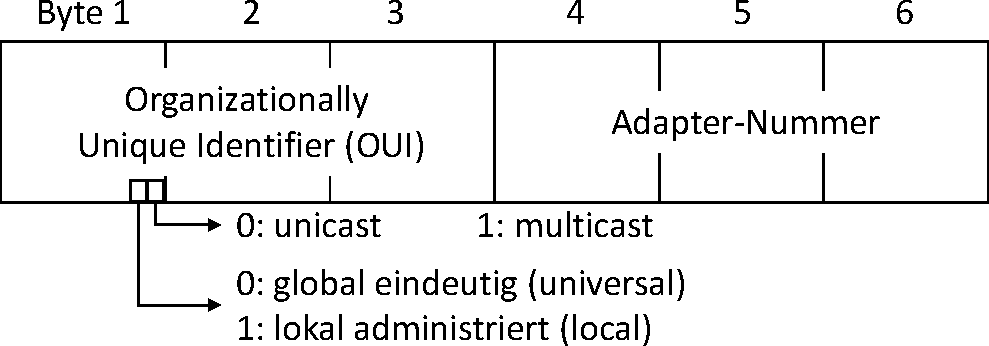
\includegraphics[width=0.7\linewidth]{Documents/MAC.pdf}
\end{center}
% ======================================================================== %
\section{Bitübertragung}
% ------------------------------------------------------------------------ %
\subsection{Betriebsweisen}
\begin{description}
	\item[Synchron] Zentraler Takt; Explizite Sendefreigabe durch den
	      Empfänger
	\item[Asynchron] Start-Stop-Erkennung notwendig; In der Regel langsamer
	      als synchron
	\item[Simplex] \(S \rightarrow E\)
	\item[Simplex mit Quittung] \(S \overset{\text{Daten}}{\longrightarrow} E \overset{\text{Quittung}}{\longrightarrow} S\)
	\item[Halbduplex] Sender und Empfänger auf beiden Seiten, teilen
	      gemeinsame Leitung
	\item[Vollduplex] Sender und Empfänger auf beiden Seiten mit eigener
	      Leitung (\(2 \cdot \text{Simplex}\))
\end{description}
% ------------------------------------------------------------------------ %
\subsubsection{Modulationsarten}
Amplitudenmodulation, Frequenzmodulation, Phasenmodulation
% ------------------------------------------------------------------------ %
\subsection{Theoretische Obergrenzen für Datenraten}
\subsubsection{Nyquist-Frequenz}
Maximale Schrittgeschwindigkeit bei einer Bandbreite \(B\)
\[V_\text{max} = 2 \cdot B\]
Maximale Datenrate in \(\frac{Bit}{s}\) bei \(L\) diskreten Stufen,
ungestört \[D_\text{max} = 2 \cdot B \cdot \log_{2}(L)\]
\subsubsection{Rauschsignal}
Umrechnung des \emph{Signal-Rausch-Abstandes} von \(dB\) in
\(\frac{\text{Signal}}{\text{Noise}}\)
\[\text{SNR} = \cfrac{\text{Signal}}{\text{Noise}}\]
\[\text{SNR [dB]} = 10 \cdot \log_{10}\left(\frac{S}{N}\right)\]
\subsubsection{Shannon-Hartley-Gesetz}
Maximale Datenrate bei bandbreitenbegrenztem, gestörten Übertragungskanal
\[D_{\text{max}} = B \cdot \log_2\left(1+\frac{S}{N}\right)\]
% ------------------------------------------------------------------------ %
\subsection{Kodierung}
\subsection{Allgemeines}
\begingroup\setlength\tabcolsep{0pt}\def\arraystretch{1.75}
\begin{center}
	\begin{tabular}{r!{\color{gray}\vline}c!{\color{gray}\vline}c!{\color{gray}\vline}c!{\color{gray}\vline}c!{\color{gray}\vline}c!{\color{gray}\vline}c!{\color{gray}\vline}c!{\color{gray}\vline}c!{\color{gray}\vline}c!{\color{gray}\vline}c!{\color{gray}\vline}c!{\color{gray}\vline}c!{\color{gray}\vline}c!{\color{gray}\vline}c!{\color{gray}\vline}c!{\color{gray}\vline}c!{\color{gray}\vline}}
		Signal~     & 0  & 0  & 1  & 0  & 1  & 1  & 1  & 1  & 0  & 1  & 0  & 0  & 0  & 0  & 1  & 0\tabularnewline
		\hline
		Takt~       & ▁█ & ▁█ & ▁█ & ▁█ & ▁█ & ▁█ & ▁█ & ▁█ & ▁█ & ▁█ & ▁█ & ▁█ & ▁█ & ▁█ & ▁█ & ▁█\tabularnewline
		NRZ~        & ▁▁ & ▁▁ & ██ & ▁▁ & ██ & ██ & ██ & ██ & ▁▁ & ██ & ▁▁ & ▁▁ & ▁▁ & ▁▁ & ██ & ▁▁\tabularnewline
		NRZI~       & ▁▁ & ▁▁ & ▁█ & ██ & █▁ & ▁█ & █▁ & ▁█ & ██ & █▁ & ▁▁ & ▁▁ & ▁▁ & ▁▁ & ▁█ & ██\tabularnewline
		Manchester~ & ▁█ & ▁█ & █▁ & ▁█ & █▁ & █▁ & █▁ & █▁ & ▁█ & █▁ & ▁█ & ▁█ & ▁█ & ▁█ & █▁ & ▁█\tabularnewline
	\end{tabular}
\end{center}
\endgroup
\begin{itemize}
	\item \textbf{N}on-\textbf{R}eturn to \textbf{Z}ero:\\
	      \(0\text{-Bit} \rightarrow \text{LOW}\)\\
	      \(1\text{-Bit} \rightarrow \text{HIGH}\)
	\item \textbf{N}on-\textbf{R}eturn to \textbf{Z}ero \textbf{I}nverted:\par
	      \(0\text{-Bit} \rightarrow \text{Widerholung des letzten Signals}\) \\
	      \(1\text{-Bit} \rightarrow \text{Änderung des Signals (Mittig zwischen)}\) \\
\end{itemize}
\paragraph{Manchester-Kodierung} Ist ein XOR von \textit{NRZ} und \textit{Takt},
\textbf{Vorteil}: in jedem Takt ein Wechsel
\textbf{Nachteil}: die Änderungsrate der Signalwechsel verdoppelt sich \\
Manchester: Bitrate = Baudrate/2; NRZ, NRZI: Bitrate = Baudrate
\subsection{AMI-Code (Alternate Mark Inversion)}
0-Bit \(\Rightarrow\) 0-Signal \\
1-Bit \(\Rightarrow\) 1- oder -1-Signal, Wechsel gegenüber dem letzten 1-Bit
\subsubsection{B8ZS-Code}
\begingroup
\setlength{\columnseprule}{0pt}
\setlength{\columnsep}{0.5\linewidth} 
\begin{multicols}{2}
	\begin{itemize}
		\item Jeweils acht 0-Bits werden durch Code-Verletzungen kodiert
		\item Sonst wie AMI
	\end{itemize}
	
\end{multicols}
\endgroup
\subsubsection{HDB3-Code}
\end{multicols*}
\end{document}
